\chapter{Bonustest 1 - Rechnen mit Vektoren}

\section{Frage 1}
Wie viele verschiedene Vektoren sind auf diesem Bild zu sehen?

In dieser Aufgabe geht es im wesentlichen darum, die \textbf{verschiedenen} Pfeile zu zählen. Es ist 
hilfreich, die Vektoren in dem Graphen so zu verschieben, dass gleiche Vektoren beieinander sind. So 
muss nur noch die Anzahl der Cluster gezählt werden.

\makebox[0.5\textwidth]{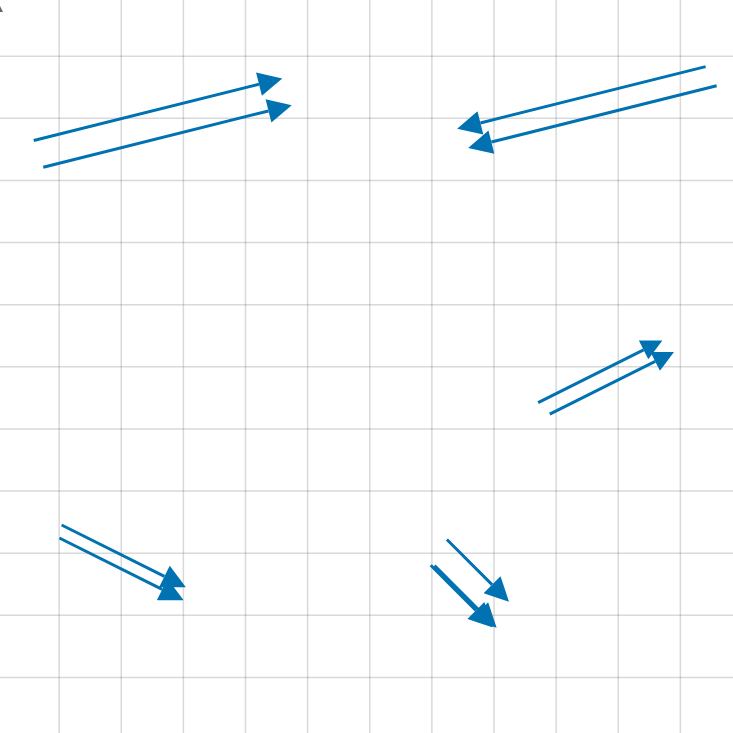
\includegraphics[width=0.5\textwidth]{bonus_tests/unique_vectors.png}}

Hier gibt es \textbf{5} verschiedene Vektoren.

\section{Frage 2}
In der folgenden Abbildung sind verschiedene Vektoren dargestellt. Ein Kästchen entspricht einer Längeneinheit.
Geben Sie die verschiedenen Vektoren, die im Bild zu sehen sind, als Liste in eckigen Klammern an. 
Die Einträge dieser Liste sind dabei die verschiedenen Vektoren dargestellt als Paare von Zahlen in eckigen Klammern. 
Ihre Antwort sollte also ein Ausdruck der Form [[1,3],[-2,0],[1,1]] oder [[0,3],[1,-1],[-1,1],[4,2]] etc. sein. 

Hier ist es auch wieder Sinnvoll, die Vektoren zu sortieren. Dann müssen die Vektoren nur noch abgelesen werden.
Die Vektoren werden über [x, y] benannt, wobei x der weg ist, den der Vektor nach rechts "geht" und y die höhe 
des Vektors ist.

\makebox[0.5\textwidth]{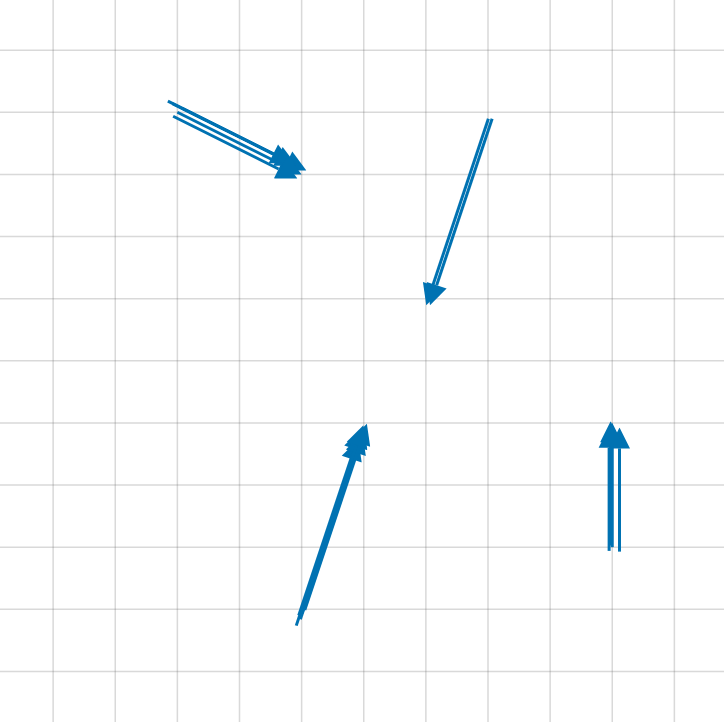
\includegraphics[width=0.5\textwidth]{bonus_tests/vector_lengths.png}}

Hier befinden sich in der Abbildung die Vektoren [[1, 3], [0, 2], [2, -1], [-1, -3]]

\section{Frage 3}
Gegeben sind im $\mathbb{R}^3$ die beiden Vektoren $\vec{u}$ und $\vec{v}$ in Komponentendarstellung,
wobei $B = (\vec{e_1}, \vec{e_2}, \vec{e_3})$ die Standardbasis des $\mathbb{R}^3$ ist.

\subsection{a}
Geben Sie die Vektoren $\vec{u}$ und $\vec{v}$ in Koordinatendarstellung an.

\subsubsection{I}
Es ist $\vec{u} = \frac{3\vec{e_3}}{2} + 2\vec{e_2} + 3\vec{e_1}$

Hier muss der Vektor berechnet werden. Da die Vektoren $\vec{e_1}, \vec{e_2}, \vec{e_3}$ die standardvektoren sind,
ist deren Wert bekannt $\left(\vec{e_1} = \begin{pmatrix}
    1 \\ 0 \\ 0
\end{pmatrix}, \vec{e_2} = \begin{pmatrix}
    0 \\ 1 \\ 0
\end{pmatrix}, \vec{e_3} = \begin{pmatrix}
    0 \\ 0 \\ 1
\end{pmatrix}\right)$. 

Bevor das Ergebnis berechnet wird, sollte noch der Bruch aufgelöst werden: 
\begin{align*}
    \frac{3\vec{e_3}}{2} = \frac{3 \cdot \vec{e_3}}{2 \cdot 1} = \frac{3}{2} \cdot \frac{\vec{e_3}}{1} = \frac{3}{2}\vec{e_3}
\end{align*}

Jetzt können die Einheitsvektoren einfach eingesetzt werden

\begin{align*}
    \frac{3}{2} \cdot \begin{pmatrix} 0 \\ 0 \\ 1 \end{pmatrix} + 2 \cdot \begin{pmatrix} 0 \\ 1 \\ 0 \end{pmatrix} + 3 \cdot \begin{pmatrix} 1 \\ 0 \\ 0 \end{pmatrix} \\
    =  \begin{pmatrix}
        \frac{3}{2} \cdot 0 \\ \frac{3}{2} \cdot 0 \\ \frac{3}{2} \cdot 1
    \end{pmatrix} + \begin{pmatrix}
        2 \cdot 0 \\ 2 \cdot 1 \\ 2 \cdot 0
    \end{pmatrix} + \begin{pmatrix}
        3 \cdot 1 \\ 3 \cdot 0 \\ 3 \cdot 0
    \end{pmatrix} \\\pagebreak[2]
    = \begin{pmatrix}
        0 \\ 0 \\ \frac{3}{2}
    \end{pmatrix} + \begin{pmatrix}
        0 \\ 2 \\ 0
    \end{pmatrix} + \begin{pmatrix}
        3 \\ 0 \\ 0
    \end{pmatrix} \\\pagebreak[2]
    = \begin{pmatrix}
        3 \\ 2 \\ \frac{3}{2}
    \end{pmatrix}
\end{align*}

Der Vektor $\vec{u}$ ist also $\begin{pmatrix}
    3 \\ 2 \\ \frac{3}{2}
\end{pmatrix}$.

\subsubsection{II}
es ist $\vec{v} = 2\vec{e_3} + 2\vec{e_2}$.

Hier können wieder die Einheitsvektoren eingesetzt werden.

\begin{align*}
    2 \cdot \begin{pmatrix}
        0 \\ 0 \\ 1
    \end{pmatrix} + 2 \cdot \begin{pmatrix}
        0 \\ 1 \\ 0
    \end{pmatrix} \\
    = \begin{pmatrix}
        2 \cdot 0 \\ 2 \cdot 0 \\ 2 \cdot 1
    \end{pmatrix} + \begin{pmatrix}
        2 \cdot 0 \\ 2 \cdot 1 \\ 2 \cdot 0
    \end{pmatrix} \\
    = \begin{pmatrix}
        0 \\ 0 \\ 2
    \end{pmatrix} + \begin{pmatrix}
        0 \\ 2 \\ 0
    \end{pmatrix} \\
    = \begin{pmatrix}
        0 \\ 2 \\ 2
    \end{pmatrix}
\end{align*}

\subsection{b}
Berechnen Sie für die Vektoren $\vec{u}$ und $\vec{v}$ aus Teilaufgabe a folgende Größen.
Geben Sie die Lösung exakt, also nicht näherungsweise an.

\subsubsection{I}
Es ist $\vec{u} - 2\vec{v}$

\begin{align*}
    \begin{pmatrix}
        3 \\ 2 \\ \frac{3}{2}
    \end{pmatrix} - 2 \cdot \begin{pmatrix}
        0 \\ 2 \\ 2
    \end{pmatrix} \\
    = \begin{pmatrix}
        3 \\ 2 \\ \frac{3}{2}
    \end{pmatrix} - \begin{pmatrix}
        0 \\ 4 \\ 4
    \end{pmatrix} \\
    = \begin{pmatrix}
        3 - 0\\ 2 - 4 \\ \frac{3}{2} - 4
    \end{pmatrix} \\
    = \begin{pmatrix}
        3 \\ -2 \\ -\frac{5}{2}
    \end{pmatrix}
\end{align*}

\subsubsection{II}
Es ist $\left|3\vec{u} + 3\vec{v}\right|$

Die Betragsstriche meinen hier, dass die Länge des Vektors berechnet werden soll. 
Diese kann über die Formel $\sqrt{v_1^2 + v_2^2 + \dots + v_n^2}$ berechnet werden.
Es muss also zunächst der resultierende Vektor von $3\vec{u} + 3\vec{v}$ berechnet werden und 
von diesen Vektor muss dann die Länge bestimmt werden.

\begin{align*}
    \left|3 \cdot \begin{pmatrix}
        3 \\ 2 \\ \frac{3}{2}
    \end{pmatrix} + 3 \cdot \begin{pmatrix}
        0 \\ 2 \\ 2
    \end{pmatrix}\right| \\
    = \left|\begin{pmatrix}
        3 \cdot 3 \\ 3 \cdot 2 \\ 3 \cdot \frac{3}{2}
    \end{pmatrix} + \begin{pmatrix}
        3 \cdot 0 \\ 3 \cdot 2 \\ 3 \cdot 2
    \end{pmatrix}\right| \\
    = \left|\begin{pmatrix}
        9 \\ 6 \\ \frac{9}{2}
    \end{pmatrix} + \begin{pmatrix}
        0 \\ 6 \\ 6
    \end{pmatrix}\right| \\
    = \left|\begin{pmatrix}
        9 \\ 12 \\ \frac{21}{2}
    \end{pmatrix}\right| \\
    = \sqrt{9^2 + 12^2 + \frac{21}{2}^2} \\
    = \sqrt{\frac{1341}{4}}
\end{align*}

\subsubsection{III}
Es ist $\left\langle\vec{u}, \vec{v}\right\rangle$

Hier soll das Skalarprodukt berechnet werden. Das Skalarprodukt $\left\langle\vec{a}, \vec{b}\right\rangle$
berechnet sich aus $a_1 \cdot b_1 + a_2 \cdot b_2 + \dots + a_n \cdot b_n$

\begin{align*}
    \left\langle \begin{pmatrix}
        3 \\ 2 \\ \frac{3}{2}
    \end{pmatrix}, \begin{pmatrix}
        0 \\ 2 \\ 2
    \end{pmatrix}\right\rangle \\
    = 3 \cdot 0 + 2 \cdot 2 + \frac{3}{2} \cdot 2 \\
    = 0 + 4 + 3 \\
    = 7
\end{align*}

\subsubsection{IV}
Es ist $\vec{u} \times \vec{v}$

Hier soll das Kreuzprodukt berechnet werden. Das Kreuzprodukt zweier Vektoren $\vec{a}, \vec{b}$ der länge 3 lässt sich 
über $\begin{pmatrix}a_2b_3 - a_3b_2 \\ a_3b_1 - a_1b_3 \\ a_1b_2 - a_2b_1 \end{pmatrix}$

\begin{align*}
    \begin{pmatrix}
        3 \\ 2 \\ \frac{3}{2}
    \end{pmatrix} \times \begin{pmatrix}
        0 \\ 2 \\2
    \end{pmatrix} \\
    = \begin{pmatrix}
        2 \cdot 2 - \frac{3}{2} \cdot 2 \\ \frac{3}{2} \cdot 0 - 3 \cdot 2 \\ 3 \cdot 2 - 2 \cdot 0
    \end{pmatrix} \\
    = \begin{pmatrix}
        4 - 3 \\ 0 - 6 \\ 6 - 0
    \end{pmatrix} \\
    = \begin{pmatrix}
        1 \\ -6 \\ 6
    \end{pmatrix}
\end{align*}

\section{Frage 4}
In welchem der folgenden Bilder ist das Skalarprodukt $\left\langle \vec{a}, \vec{b} \right\rangle$ negativ?

Das Skalarprodukt zweier Vektoren ist negativ, wenn der Winkel zwischen den Vektoren größer als 90° beträgt.

\subsection*{Herleitung: Vorzeichen des Skalarprodukts}
Das Skalarprodukt zweier Vektoren $\vec{a}$ und $\vec{b}$ ist fundamental durch ihre Beträge und den von ihnen 
eingeschlossenen Winkel $\theta$ definiert:
$$ \left\langle \vec{a}, \vec{b} \right\rangle = |\vec{a}| \cdot |\vec{b}| \cdot \cos(\theta) $$
Hierbei sind $|\vec{a}|$ und $|\vec{b}|$ die Längen der Vektoren. Der Winkel $\theta$ ist der 
kleinste Winkel zwischen $\vec{a}$ und $\vec{b}$, sodass $0^\circ \le \theta \le 180^\circ$.

\subsubsection*{Die Rolle des Kosinus}
Die Beträge $|\vec{a}|$ und $|\vec{b}|$ sind per Definition stets nicht-negativ. Wenn wir annehmen, 
dass weder $\vec{a}$ noch $\vec{b}$ der Nullvektor ist (d.h. $|\vec{a}| > 0$ und $|\vec{b}| > 0$), dann 
sind ihre Beträge positive Zahlen.
Das Produkt zweier positiver Zahlen ($|\vec{a}| \cdot |\vec{b}|$) ist ebenfalls positiv.
Folglich hängt das Vorzeichen des gesamten Skalarprodukts $\left\langle \vec{a}, \vec{b} \right\rangle$ 
ausschließlich vom Vorzeichen des Terms $\cos(\theta)$ ab:
$$ \text{Vorzeichen}(\left\langle \vec{a}, \vec{b} \right\rangle) = \text{Vorzeichen}(\cos(\theta)) $$

\subsubsection*{Verhalten von $\cos(\theta)$ im relevanten Winkelbereich}
Betrachten wir das Vorzeichen von $\cos(\theta)$ für die möglichen Werte des Winkels $\theta$ zwischen zwei Vektoren:
\begin{itemize}
    \item \textbf{Spitzer Winkel:} $0^\circ \le \theta < 90^\circ$
    
    Für Winkel in diesem Bereich ist der Kosinus positiv: $\cos(\theta) > 0$.
    Das Skalarprodukt ist somit:
    $$ \left\langle \vec{a}, \vec{b} \right\rangle = \underbrace{|\vec{a}| \cdot |\vec{b}|}_{\text{positiv}} 
    \cdot \underbrace{\cos(\theta)}_{\text{positiv}} \quad \implies \quad \left\langle \vec{a}, \vec{b} 
    \right\rangle > 0 $$
    
    \item \textbf{Rechter Winkel:} $\theta = 90^\circ$
    
    Für einen rechten Winkel ist der Kosinus Null: $\cos(90^\circ) = 0$.
    Das Skalarprodukt ist somit:
    $$ \left\langle \vec{a}, \vec{b} \right\rangle = |\vec{a}| \cdot |\vec{b}| \cdot 
    \underbrace{\cos(90^\circ)}_{0} \quad \implies \quad \left\langle \vec{a}, \vec{b} \right\rangle = 0 $$
    In diesem Fall stehen die Vektoren orthogonal (senkrecht) aufeinander.
    
    \item \textbf{Stumpfer Winkel:} $90^\circ < \theta \le 180^\circ$
    
    Für Winkel in diesem Bereich ist der Kosinus negativ: $\cos(\theta) < 0$.
    Das Skalarprodukt ist somit:
    $$ \left\langle \vec{a}, \vec{b} \right\rangle = \underbrace{|\vec{a}| \cdot |\vec{b}|}_{\text{positiv}} 
    \cdot \underbrace{\cos(\theta)}_{\text{negativ}} \quad \implies \quad \left\langle \vec{a}, \vec{b} 
    \right\rangle < 0 $$
\end{itemize}

\subsubsection*{Schlussfolgerung aus der Herleitung}
Das Skalarprodukt $\left\langle \vec{a}, \vec{b} \right\rangle$ ist \textbf{genau dann negativ}, wenn der 
Kosinus des von den Vektoren eingeschlossenen Winkels $\theta$ negativ ist. Dies ist der Fall, wenn der 
Winkel $\theta$ ein stumpfer Winkel ist, also $90^\circ < \theta \le 180^\circ$.

\section{Frage 5}

Gegeben sind zwei $\mathbb{R}^3$-Vektoren

\[
\vec{a} = \begin{pmatrix}
    -\frac{3}{2} \\
    \frac{8}{3} \\
    1
\end{pmatrix} \quad \vec{b} = \begin{pmatrix}
    1 \\ 0 \\ \frac{8}{3}
\end{pmatrix}
\]

Bestimmen Sie den Winkel zwischen $a$ und $b$ und runden diesen auf zwei Dezimalstellen genau in Grad und Bogenmaß.

\subsection{a}

Der Winkel zwischen zwei Vektoren kann berechnet werden, über $\cos(\theta) = \frac{\left\langle \vec{a}, \vec{b} \right\rangle}{\left|\vec{a}\right| \cdot \left|\vec{b}\right|}$. Hier müssen ganz einfach die Vektoren eingesetzt werden

\begin{align*}
    \cos(\theta) = \frac{\left\langle \vec{a}, \vec{b} \right\rangle}{\left|\vec{a}\right| \cdot \left|\vec{b}\right|} \\\\
    \left\langle \vec{a}, \vec{b} \right\rangle = -\frac{3}{2} \cdot 1 + \frac{8}{3} \cdot 0 + 1 \cdot \frac{8}{3} \\
    = -\frac{3}{2} + \frac{8}{3} \\
    = \frac{7}{6} \\\\
    \left|a\right| = \sqrt{{(-\frac{3}{2})}^2 + \frac{8}{3}^2 + 1^2} \\
    = \sqrt{{\frac{9}{4}} + \frac{64}{9} + 1}
    = \sqrt{\frac{373}{36}} \\\\
    \left|b\right| = \sqrt{1^2 + 0^2 + \frac{8}{3}^2} \\
    = \sqrt{1 + 0 + \frac{64}{9}}
    = \sqrt{\frac{73}{9}} \\\\
    \cos(\theta) = \frac{\frac{7}{6}}{\sqrt{\frac{373}{36}} \cdot \sqrt{\frac{73}{9}}} = \frac{21 \sqrt{27229}}{27229} \\
    \arccos\left(\frac{21 \sqrt{27229}}{27229}\right) \approx 1.44 rad \\
    \arccos\left(\frac{21 \sqrt{27229}}{27229}\right) \cdot \frac{180}{\pi} \approx 82.71^\circ
\end{align*}

Der Winekl zwischen den gegebenen Vektoren beträgt in Gradmaß $\theta_{grad}$ = $82.71$.

\subsection{b}

Der Winkel zwischen den gegebenen Vektoren beträgt in Bogenmaß $\theta_{Bogen}$ = $1.44$.

\section{Frage 6}

Gegeben sind die zwei Ortsvektoren
\[
    \vec{u} = \begin{pmatrix}
        5 \\ -1 \\ 4
    \end{pmatrix}, \quad \vec{v} = \begin{pmatrix}
        -1 \\ 0 \\ -2
    \end{pmatrix} \text{ der beiden Punkte } U \text{ und } V\text{.}
\]

\subsection{a}

Wie in der folgenden Abbildung dargestellt, unterteilen die Punkte $U$ und $V$ die Strecke von Punkt $X$ zu Punkt $Y$ in drei gleich lange Teile.

\begin{center}
\begin{tikzpicture}[
    punkt/.style={circle, fill, inner sep=1.5pt},
  ]

  \coordinate (x) at (0, 0);
  \coordinate (y) at (7, 1.5);

  \draw[cyan, line width=1.2pt] (x) -- (y);

  \node[punkt, cyan, label=below left:$X$] at (x) {};
  \node[punkt, cyan, label=above right:$Y$] at (y) {};

  \path (x) -- (y) coordinate[pos=1/3] (u) coordinate[pos=2/3] (v);

  \draw[black, line width=1.2pt] (u) -- (v);

  \node[punkt, black, label=above:$U$] at (u) {};
  \node[punkt, black, label=above:$V$] at (v) {};
\end{tikzpicture}
\end{center}

Bestimmen Sie die Ortsvektoren $\vec{x}$ und $\vec{y}$ der Punkte $X$ und $Y$.

\subsubsection{Lösung}
Der Verbindungsvektor von Punkt $U$ nach Punkt $V$ lässt sich aus den zugehörigen Ortsvektoren $\vec{u}$ und $\vec{v}$ berechnen:
\begin{align*}
    \vec{UV} &= \vec{v} - \vec{u} \\
    &= \begin{pmatrix}
        -1 \\ 0 \\ -2
    \end{pmatrix} - \begin{pmatrix}
        5 \\ -1 \\ 4
    \end{pmatrix} \\
    &= \begin{pmatrix}
        -6 \\ 1 \\ -6
    \end{pmatrix}
\end{align*}
Da die Strecke in drei gleich lange Teile unterteilt ist, gilt $\vec{XU} = \vec{UV} = \vec{VY}$.
\newline
\newline
Der Ortsvektor $\vec{x}$ des Punktes $X$ kann somit durch Subtraktion des Vektors $\vec{UV}$ vom Ortsvektor $\vec{u}$ bestimmt werden:
\begin{align*}
    \vec{x} &= \vec{u} - \vec{UV} \\
    &= \begin{pmatrix}
        5 \\ -1 \\ 4
    \end{pmatrix} - \begin{pmatrix}
        -6 \\ 1 \\ -6
    \end{pmatrix} \\
    &= \begin{pmatrix}
        11 \\ -2 \\ 10
    \end{pmatrix}
\end{align*}
Analog ergibt sich der Ortsvektor $\vec{y}$ des Punktes $Y$ aus der Addition des Vektors $\vec{UV}$ zum Ortsvektor $\vec{v}$:
\begin{align*}
    \vec{y} &= \vec{v} + \vec{UV} \\
    &= \begin{pmatrix}
        -1 \\ 0 \\ -2
    \end{pmatrix} + \begin{pmatrix}
        -6 \\ 1 \\ -6
    \end{pmatrix} \\
    &= \begin{pmatrix}
        -7 \\ 1 \\ -8
    \end{pmatrix}
\end{align*}

\subsection{b}

Bestimmen Sie die Ortsvektoren $\vec{x}$ und $\vec{y}$ als Linearkombination von $\vec{u}$ und $\vec{v}$.

\subsubsection*{Lösung}
Aus Teil a sind die Beziehungen $\vec{x} = \vec{u} - \vec{UV}$ und $\vec{y} = \vec{v} + \vec{UV}$ bekannt, sowie $\vec{UV} = \vec{v} - \vec{u}$. Durch Einsetzen von $\vec{UV}$ lässt sich $\vec{x}$ als Linearkombination von $\vec{u}$ und $\vec{v}$ darstellen:
\begin{align*}
    \vec{x} &= \vec{u} - (\vec{v} - \vec{u}) \\
    &= \vec{u} - \vec{v} + \vec{u} \\
    &= 2\vec{u} - \vec{v}
\end{align*}
Ebenso für $\vec{y}$:
\begin{align*}
    \vec{y} &= \vec{v} + (\vec{v} - \vec{u}) \\
    &= \vec{v} + \vec{v} - \vec{u} \\
    &= 2\vec{v} - \vec{u}
\end{align*}
Die gesuchten Linearkombinationen lauten somit:
\[
    \vec{x} = 2\vec{u} - \vec{v} \quad \text{und} \quad \vec{y} = - \vec{u} + 2\vec{v}
\]

\section{Frage 7}

Auf einem Billardtisch befinden sich eine blaue und eine weiße Kugel. Die weiße Kugel und die blaue Kugel haben beide einen Durchmesser \(d = 57.2\,\text{mm}\). In der folgenden Abbildung ist der Billardtisch dargestellt. Der Punkt \(A\) bezeichnet den Mittelpunkt der weißen Kugel und der Punkt \(B\) den Mittelpunkt der blauen Kugel. Die Punkte liegen jeweilts auf einem Gitterpunkt des quadratischen Rasters, wobei ein Kästchen eine skalierung von \(1\,\text{dm}\) hat. Die obere rechte Tasche des Billarftisches wird mit \(C\) und die untere rechte Tasche mit \(D\) bezeichnet.

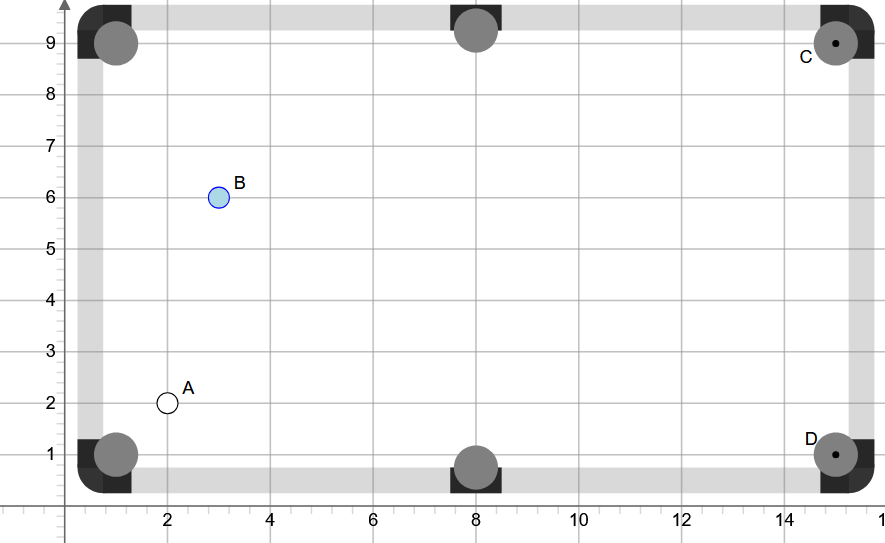
\includegraphics[width=\textwidth]{bonus_tests/pool.png}

Hier ist die Kugel B bei \(\begin{pmatrix} 3 \\ 6 \end{pmatrix}\) und die Kugel A bei \(\begin{pmatrix} 2 \\ 2 \end{pmatrix}\).

Die weiße Kugel wird so gespielt, dass die blaue Kugel danach direkt zu Punkt \(C\) rollt. Die folgende Abbildung zeigt die weiße und blaue Kugel beim Stoß. Dabei ist \(A'\) die Position der weißen Kugel, wenn diese auf die blaue Kugel trifft. Der Impuls wird hierbei entlang der Linie \(A'B\) übertragen.

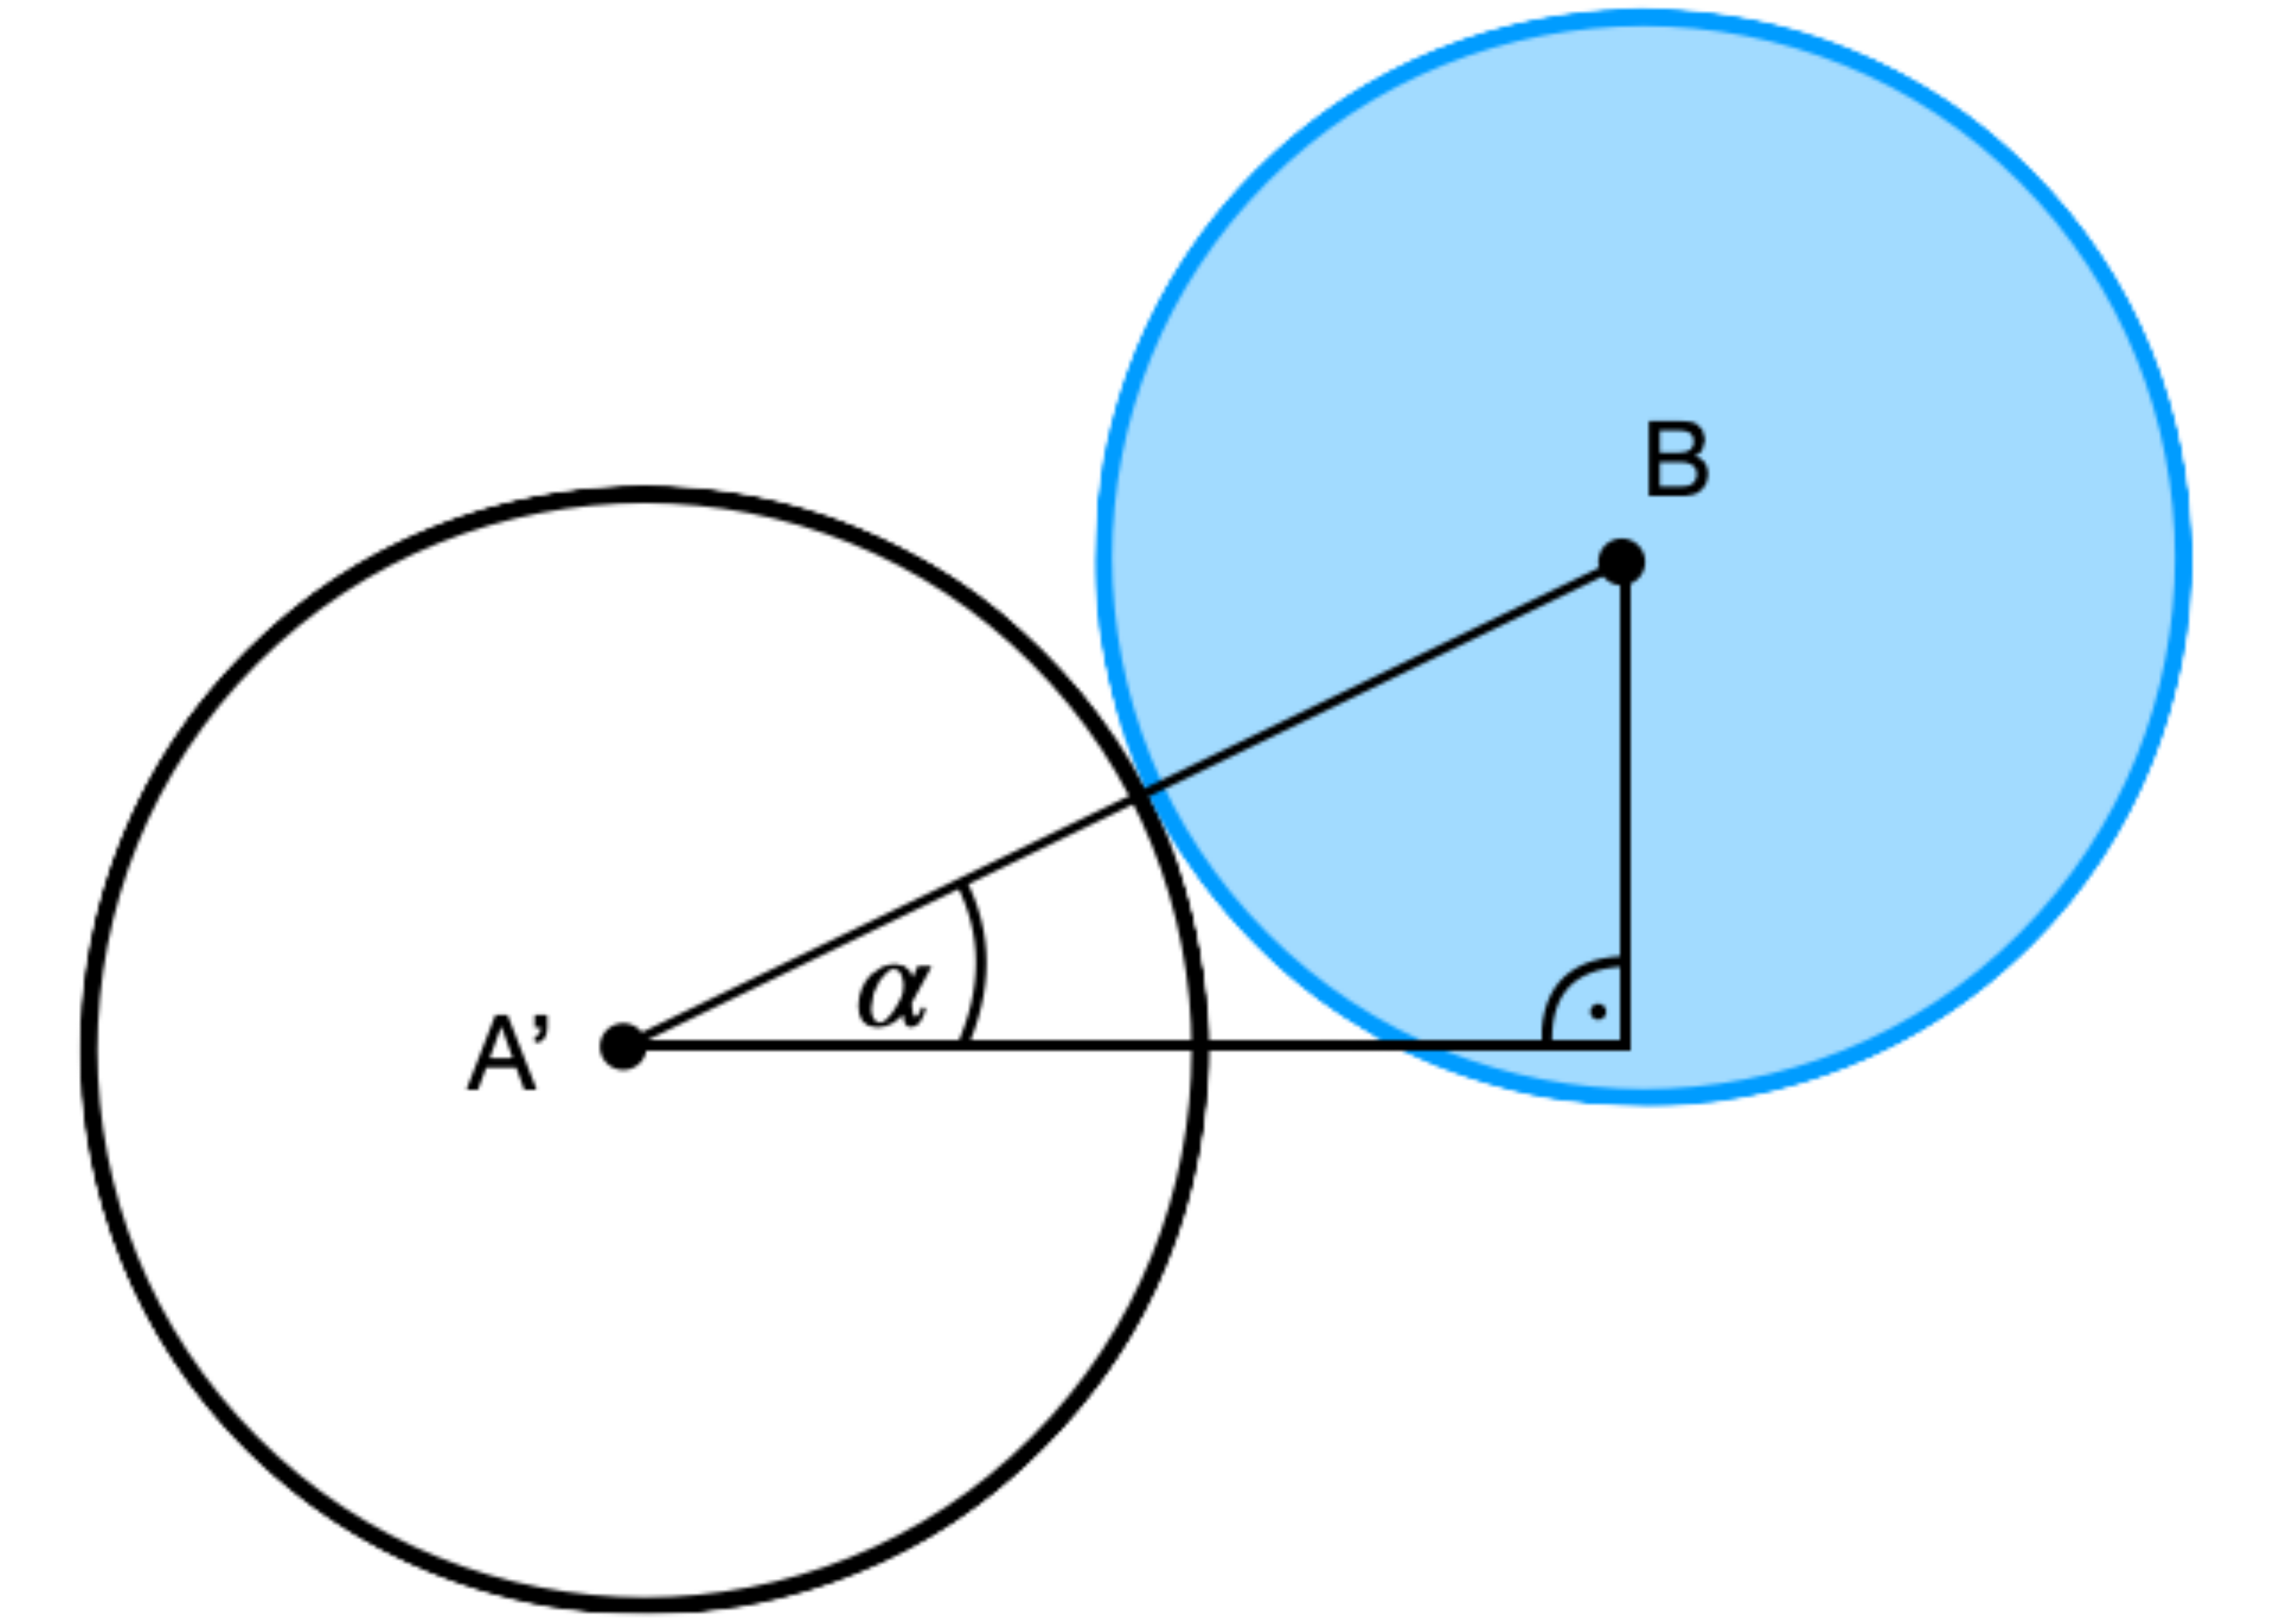
\includegraphics[width=\textwidth]{bonus_tests/pool2.png}

\subsection{a}

Berechnen Sie den Winkel \(\alpha\), unter dem die weiße Kugel die blaue Kugel treffen muss, damit die blaue Kugel direkt in Loch \(C\) trifft. Geben Sie den Winkel in Gradmaß und auf zwei Dezimalstellen genau ein.

Der Richtungsvektor der blauen Kugel ist \(\vec{BC}\).
\[
\vec{BC} = \vec{C} - \vec{B} = \begin{pmatrix} 15 \\ 9 \end{pmatrix} - \begin{pmatrix} 3 \\ 6 \end{pmatrix} = \begin{pmatrix} 12 \\ 3 \end{pmatrix}
\]
Der Winkel \(\theta\) dieses Vektors zur x-Achse \(\begin{pmatrix} 1 \\ 0 \end{pmatrix}\) ist:
\begin{align*}
    \cos(\theta) &= \frac{\begin{pmatrix} 12 \\ 3 \end{pmatrix} \cdot \begin{pmatrix} 1 \\ 0 \end{pmatrix}}{|\begin{pmatrix} 12 \\ 3 \end{pmatrix}| \cdot |\begin{pmatrix} 1 \\ 0 \end{pmatrix}|} = \frac{12}{\sqrt{12^2 + 3^2} \cdot \sqrt{1^2}} = \frac{12}{\sqrt{153}} \\
    \theta &= \arccos\left(\frac{12}{\sqrt{153}}\right) \approx 14.04^\circ
\end{align*}

\subsection{b}
Berechnen Sie den Vektor \(\vec{A'B}\) in dm und auf zwei Dezimalstellen genau.

Der Vektor \(\vec{A'B}\) verläuft vom Zentrum der weißen Kugel (\(A'\)) zum Zentrum der blauen Kugel (\(B\)) im Moment des Stoßes. Er hat die Richtung von \(\vec{BC}\) und die Länge des Kugeldurchmessers \(d = 0.572\,\text{dm}\).
\begin{align*}
    \vec{A'B} &= d \cdot \frac{\vec{BC}}{|\vec{BC}|} = 0.572 \cdot \frac{1}{\sqrt{153}}\begin{pmatrix} 12 \\ 3 \end{pmatrix} \\
    &\approx 0.572 \cdot \begin{pmatrix} 0.9701 \\ 0.2425 \end{pmatrix} \approx \begin{pmatrix} 0.55 \\ 0.14 \end{pmatrix}
\end{align*}

\subsection{c}

Bestimmen Sie den Vektor \(\vec{AA'}\), in dessen Richtung die weiße Kugel gespielt wird, in dm und auf zwei Dezimalstellen genau.

Zuerst wird die Position von \(A'\) bestimmt: \(\vec{A'} = \vec{B} - \vec{A'B}\).
\begin{align*}
    \vec{A'} &\approx \begin{pmatrix} 3 \\ 6 \end{pmatrix} - \begin{pmatrix} 0.55 \\ 0.14 \end{pmatrix} = \begin{pmatrix} 2.45 \\ 5.86 \end{pmatrix}
\end{align*}
Der Vektor der Stoßrichtung \(\vec{AA'}\) ist dann \(\vec{A'} - \vec{A}\).
\begin{align*}
    \vec{AA'} &\approx \begin{pmatrix} 2.45 \\ 5.86 \end{pmatrix} - \begin{pmatrix} 2 \\ 2 \end{pmatrix} = \begin{pmatrix} 0.45 \\ 3.86 \end{pmatrix}
\end{align*}

\subsection{d}
Berechnen Sie den Winkel \(\beta\) zwischen dem Stoßvektor \(\vec{AA'}\) und der Horizontalen.

Der gesuchte Winkel \(\beta\) ist der Winkel zwischen dem Stoßvektor \(\vec{AA'}\) und der horizontalen Achse.
\begin{align*}
    \cos(\beta) &= \frac{\vec{AA'} \cdot \begin{pmatrix} 1 \\ 0 \end{pmatrix}}{|\vec{AA'}| \cdot |\begin{pmatrix} 1 \\ 0 \end{pmatrix}|} \\
    \vec{AA'} \cdot \begin{pmatrix} 1 \\ 0 \end{pmatrix} &\approx 0.45 \cdot 1 + 3.86 \cdot 0 = 0.45 \\
    |\vec{AA'}| &\approx \sqrt{0.45^2 + 3.86^2} = \sqrt{0.2025 + 14.8996} = \sqrt{15.1021} \approx 3.886 \\
    |\begin{pmatrix} 1 \\ 0 \end{pmatrix}| &= 1 \\
    \cos(\beta) &\approx \frac{0.45}{3.886 \cdot 1} \approx 0.1158 \\
    \beta &= \arccos(0.1158) \approx 83.35^\circ
\end{align*}
Der gesuchte Winkel beträgt also \(83.35^\circ\).

\section{Frage 8}

Auf einem Körper, der den Punkt $O$ drehbar ist, wirkt eine am Punkt $R$ angreifende Kraft $\vec{F}$. Der vektor $\vec{r}$ ist der Ortsvektor von Punkt $O$ nach Punkt $R$. In der folgenden Abbildung ist der Körper dargestellt.

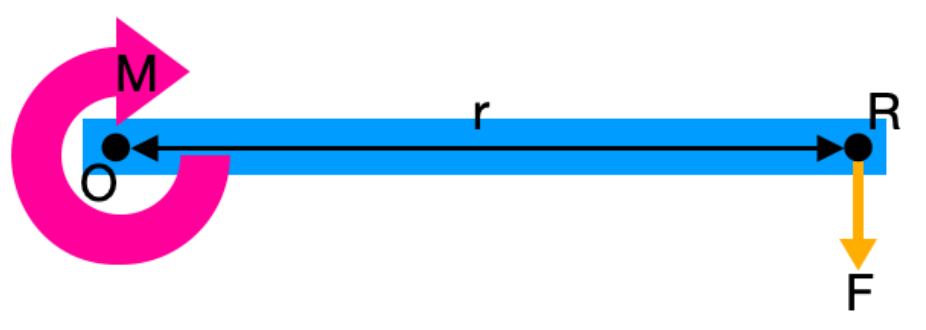
\includegraphics[width=\textwidth]{bonus_tests/drehmoment.png}


Das auf den Körper wirkende Drehmoment $\vec{M}$ ist das Kreuzprodukt $\vec{M} = \vec{r} \times \vec{F}$.

Im folgenden sei $\vec{r} = \begin{pmatrix}
        4 \\ 2 \\ -1
    \end{pmatrix}$ und $\vec{F} = \begin{pmatrix}
        2 \\ -3 \\ -6
    \end{pmatrix}$.

\subsection{a}
Berechnen Sie das auf den Körper wirkende Drehmoment $\vec{M}$.

\begin{align*}
    \vec{M} = \vec{r} \times \vec{F} \\
    = \begin{pmatrix}
        4 \\ 2 \\ -1 
    \end{pmatrix} \times \begin{pmatrix}
        2 \\ -3 \\ -6
    \end{pmatrix} \\
    = \begin{pmatrix}
        2 \cdot -6 - -1 \cdot -3 \\
        -1 \cdot 2 - 4 \cdot -6 \\
        4 \cdot -3 - 2 \cdot 2
    \end{pmatrix} \\
    \begin{pmatrix}
        -12 - 3 \\
        -2 - -24 \\
        -12 -4
    \end{pmatrix} \\
    \begin{pmatrix}
        -15 \\
        22 \\
        -16
    \end{pmatrix}
\end{align*}

\subsection{b}

Berechnen Sie den Betrag des Drehmoments und geben Sie das ergebnsi exakt an. 

\begin{align*}
    \left|\vec{M}\right| \\
    = \left|\begin{pmatrix}
        -15 \\ 22 \\ -16
    \end{pmatrix}\right| \\
    = \sqrt{-15^2 + 22^2 -16^2} \\
    = \sqrt{225 + 484 + 256} \\
    = \sqrt{965}
\end{align*}